\section{Datos Generales y gestión estratégica}

\subsection{Nombre de la empresa. Dirección}
\textbf{Nombre Comercial:} PetShop Huellitas \& Snacks \\
\textbf{Dirección Física:} Av. de los Granados N34-12 y Av. 6 de Diciembre, Edificio Plaza Norte, Planta Baja, Quito, Ecuador.

\subsection{Descripción de las actividades}
PetShop Huellitas \& Snacks es un establecimiento minorista dedicado a la comercialización de comida balanceada, galletas, snacks orgánicos y suplementos nutricionales para mascotas domésticas (perros, gatos, aves y roedores). Las actividades principales de la empresa incluyen el abastecimiento con distribuidores nacionales e importadores, la gestión física del inventario del local, la venta directa en el establecimiento físico, y la distribución de pedidos a domicilio a través de su canal de delivery rápido para el sector norte y centro de la ciudad de Quito.

\subsection{Foto de la empresa}
\begin{figure}[H]
    \centering
    % Asegúrate de que esta imagen exista en tu carpeta Images/
    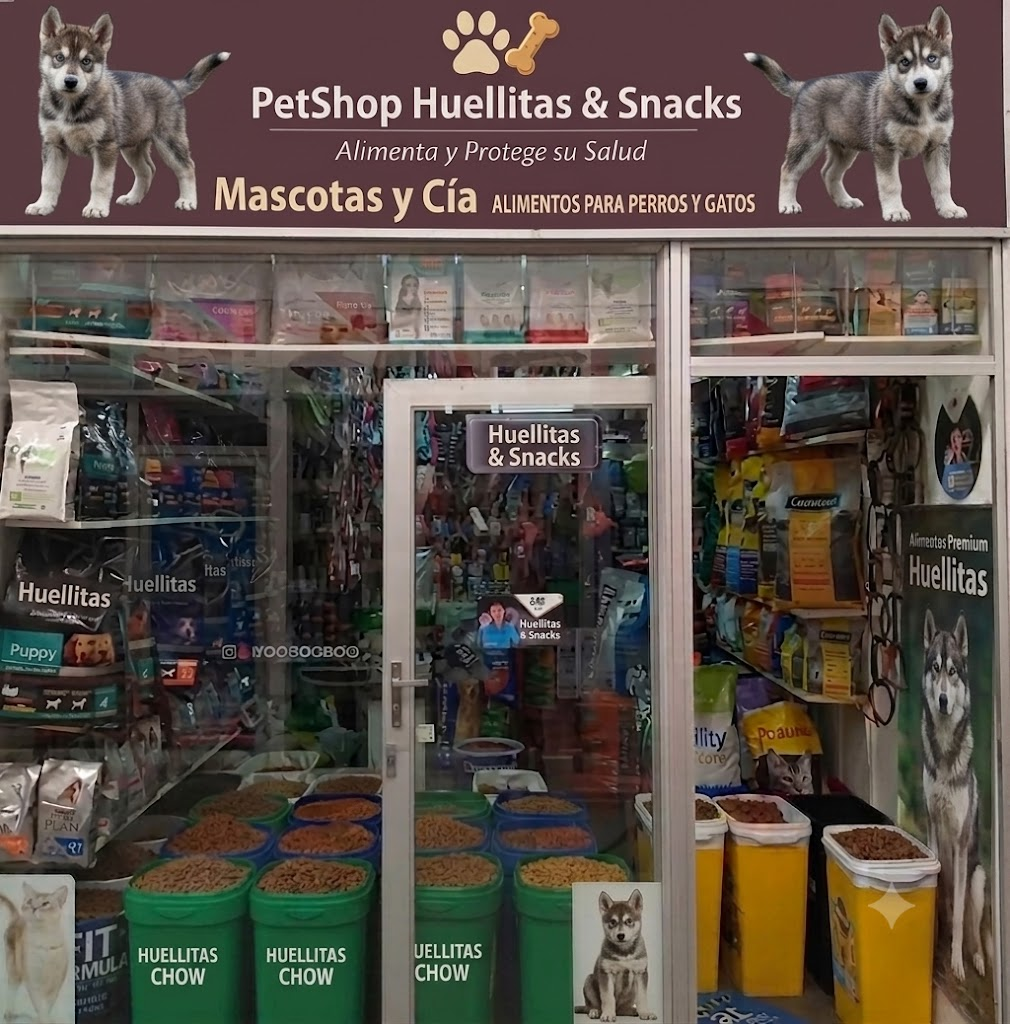
\includegraphics[width=0.70\textwidth]{Images/FotoTienda.png}
    \caption{Fachada del establecimiento de la Tienda de Comida de Mascotas}
    \label{fig:foto_empresa}
\end{figure}

\subsection{Análisis FODA}
\begin{table}[H]
    \centering
    \small
    \renewcommand{\arraystretch}{1.4}
    \begin{tabularx}{\textwidth}{|X|X|}
        \hline
        \rowcolor{upsblue} \multicolumn{2}{|c|}{\textcolor{white}{\textbf{MATRIZ FODA}}} \\
        \hline
        \rowcolor{lightgray} \textbf{Fortalezas (F)} & \textbf{Debilidades (D)} \\
        \hline
        1. Stock diverso y constante de marcas premium de alimento (Royal Canin, Hills, ProPlan) y snacks especializados. \par
        2. Servicio a domicilio establecido y consolidado en el norte y centro de la ciudad. & 
        1. Registro lento de pedidos de clientes realizados de forma manual mediante WhatsApp y canales de voz. \par
        2. Falta de consistencia e integración inmediata entre el stock físico disponible y el stock lógico registrado. \\
        \hline
        \rowcolor{lightgray} \textbf{Oportunidades (O)} & \textbf{Amenazas (A)} \\
        \hline
        1. Aumento del número de hogares de la zona con mascotas que requieren compras de alimento mensuales. \par
        2. Disposición del usuario a suscribirse a portales de envíos recurrentes programados. & 
        1. Competencia directa de supermercados de gran escala que ofertan marcas estándar a bajo costo. \par
        2. Demoras y problemas logísticos por parte de importadores mayoristas de productos premium. \\
        \hline
    \end{tabularx}
    \caption{Análisis FODA - PetShop Huellitas \& Snacks}
    \label{tab:foda}
\end{table}

\subsection{Estrategia de Supervivencia MIN-MIN}\label{sec:estrategia}
Tras el análisis de los factores de la matriz FODA, se determinó que el proyecto debe guiarse por la \textbf{Estrategia de Supervivencia (MIN-MIN)} para contrarrestar las debilidades internas y resistir a las amenazas externas. 

El cruce de factores se realiza vinculando las debilidades de registro manual de pedidos y desorganización de inventario (D1, D2) con la amenaza de grandes supermercados competidores directos (A1). Para competir y subsistir, PetShop Huellitas \& Snacks requiere implementar el sistema informático transaccional ``PetFood-Manager'' que automatice el inventario y controle el stock en tiempo real. Al suprimir errores de stock y acelerar los pedidos mediante una pasarela web ágil, el negocio optimiza sus costos operativos y previene retrasos de abastecimiento, permitiéndole mantener la fidelidad de sus clientes y asegurar su rentabilidad frente al retail masivo.

A continuación, se detalla la matriz de cruce para la formulación de las estrategias de supervivencia (MIN-MIN) en función de las amenazas externas identificadas:

\begin{table}[H]
    \centering
    \small
    \renewcommand{\arraystretch}{1.4}
    \begin{tabularx}{\textwidth}{|L|p{4cm}|L|}
        \hline
        \rowcolor{upsblue}
        \textcolor{white}{\textbf{Amenaza (Entorno)}} & 
        \textcolor{white}{\textbf{Debilidad Interna}} & 
        \textcolor{white}{\textbf{Estrategia de Supervivencia (MIN-MIN)}} \\
        \hline
        \textbf{A1: Competencia directa de supermercados de gran escala} con marcas genéricas de bajo costo. & 
        \textbf{D1:} Registro manual e ineficiente de pedidos. \par
        \textbf{D2:} Desvinculación de stock físico y lógico. & 
        \textbf{Estrategia DA1 (Sincronización Transaccional):} Implementar la pasarela de pedidos y catálogo web en el sistema ``PetFood-Manager'' enlazado en tiempo real al inventario. Al acelerar la facturación y el delivery propio, se retiene a los clientes mediante excelencia en servicio frente al retail masivo. \\
        \hline
        \textbf{A2: Demoras logísticas de importadores} en abastecer marcas premium. & 
        \textbf{D2:} Falta de control preventivo de existencias. & 
        \textbf{Estrategia DA2 (Alertas Tempranas):} Configurar límites de stock mínimo por alimento en el catálogo que disparen alertas automáticas de compra al proveedor. Esto permite realizar pedidos con anticipación, previniendo quiebres de stock ante demoras de importación. \\
        \hline
    \end{tabularx}
    \caption{Matriz de Estrategias de Supervivencia MIN-MIN por Amenazas}
    \label{tab:estrategias_minmin}
\end{table}